\documentclass[a4paper, oneside]{article}
\usepackage[utf8]{inputenc}
\usepackage[ngerman]{babel}
\usepackage[top=2.5cm, bottom=3cm, outer=2.5cm, inner=2.5cm, heightrounded]{geometry}
\usepackage{graphicx}
\usepackage{morefloats}
\usepackage{wrapfig}
\usepackage{hyperref}
\usepackage{cite}
\usepackage{siunitx}
\usepackage[default]{sourcesanspro}
\usepackage[T1]{fontenc}
\usepackage{url}
\usepackage{marginnote}
\usepackage[font=footnotesize]{caption}
\usepackage{color}
\usepackage{xcolor}
\usepackage{multicol}
\usepackage[fleqn]{mathtools}
\usepackage{amssymb}
\usepackage{wrapfig}
\usepackage[noindentafter]{titlesec}
\usepackage{fancyhdr}
\usepackage{lastpage}
\usepackage{comment}

%% LÖSUNGEN ANZEIGEN
\newif\ifshow
%\showtrue
\showfalse

%%%SECTIONING
\renewcommand*{\marginfont}{\noindent\rule{0pt}{0.7\baselineskip}\footnotesize}

\newcommand{\aufgabe}[1]{\subsection{#1}}
\newcommand{\loesung}[1]{\subsubsection{#1}}

\newcommand{\simpleset}[1]{\ensuremath \left\{ #1 \right\}}
\newcommand{\ematrix}[2]{\renewcommand{\arraystretch}{1}\ensuremath\left(\begin{array}{@{}#1@{}}#2\end{array}\right)}

\renewcommand{\theenumi}{\alph{enumi})}
\renewcommand{\labelenumi}{\text{\theenumi}}

\newcounter{aufgabe}
%\newenvironment{lsg}{\loesung}{}
\ifshow
  \newenvironment{lsg}{\loesung}{}
\else
  \excludecomment{lsg}
\fi

\newenvironment{inhalt}
  {\paragraph{Inhalt des Übungsblatts:}\itemize\let\origitem\item}
  {\enditemize\vspace{2em}}

\newcommand{\R}{\ensuremath\mathbb{R}}
\newcommand{\N}{\ensuremath\mathbb{N}}
\newcommand{\Z}{\ensuremath\mathbb{Z}}
\newcommand{\LM}{\ensuremath\mathbb{L}}
\newcommand{\intd}{\ensuremath\mathrm{d}}
\newcommand{\e}{\ensuremath\mathrm{e}}
\renewcommand{\d}{\,\mathrm{d}}
\newcommand{\stf}[1]{\ensuremath \left[ #1 \right]}

\newcommand{\cas}{\hfill (CAS)}
\newcommand{\seite}[1]{\textit{(S. #1)}}

\newcommand{\vektor}[1]{\ensuremath\begin{pmatrix} #1 \end{pmatrix}}


\everymath{\displaystyle}

%Malpunkte
\mathcode`\*="8000
{\catcode`\*\active\gdef*{\cdot}}

%SECTION
\titleformat{\section}
{\clearpage\setcounter{aufgabe}{0}\vspace{1em}\Large\raggedright\bfseries}
{}
{0pt}
{}

\titleformat{\subsection}[runin]
{\stepcounter{aufgabe}\vspace{1px}\normalfont\raggedright\bfseries}
{A\theaufgabe: }
{0pt}
{\ }

\titleformat{\subsubsection}[runin]
{\normalfont\raggedright\bfseries}
{Lösung \theaufgabe: }
{0pt}
{\ }


%FANCYHDR
\pagestyle{fancy}
\lhead{\small Simon König\\ Joshua Fabian}
\rhead{\small Mathecrashkurs 2018}
\cfoot{Seite \thepage\thinspace von\thinspace\pageref{LastPage}}
\lfoot{}
\renewcommand{\headrulewidth}{0.5pt}
\renewcommand{\footrulewidth}{0pt}

\title{Mathe-Crashkurs 2018 - Übungsblatt}
\date{\today}
\author{Simon König, Joshua Fabian}

\chead{\Large Übungsblatt 1}

\begin{document}
\begin{inhalt}
	\item Extremstellen und -Punkte \seite{29}
	\item Exponentialfunktion, Logarithmus \seite{33}
	\item Funktionenscharen \seite{35}
  \item Integral \seite{37}, Rotationskörper \seite{40}, Flächeninhalte \seite{41}
	\item Funktionsanalyse \seite{45}, gebrochenrationale Funktionen, Asymptoten \seite{46}
\end{inhalt}

\aufgabe{Gleichung lösen}
Löse die Gleichung $\e^{5x}-\e^{3x}=6\e^x$.\\
\textit{Hinweis: Du brauchst ungefähr alle gelernten Methoden!}
\begin{lsg}{}
	\begin{multicols}{2}
	\begin{align*}
		\e^{5x}-\e^{3x}&=6\e^x &&|-6\e^x\\
		\e^{5x}-\e^{3x}-6\e^x&=0 &&|\ \text{Ausklammern}\\
		\e^x\cdot(\e^{4x}-\e^{2x}-6)&=0 &&|\ \text{Nullprodukt und Substitution: } z=\e^{2x}\\
		z^2-z-6&=0 &&|\ \text{Mitternachtsformel}\\
		z_1=-2 \quad z_2&=3&&|\ \text{Resubstitution: } z_{1/2}=\e^{2\cdot x_{1/2}}\\
		\e^{2\cdot x_1}&=-2 &&\Rightarrow \text{nicht möglich ($\e^x$ immer $>0$)}\\
		\e^{2\cdot x_2}&= 3 &&\rightsquigarrow x=\frac{\ln(3)}{2}
	\end{align*}
	\end{multicols}
\end{lsg}



\aufgabe{Graphanalyse: } (vgl. Abitur 2015)
\begin{multicols}{2}
	Die Abbildung zeigt den Graphen der Ableitungsfunktion $f'$ einer ganzrationalen Funktion $f$.
	Entscheiden Sie ob die folgenden Aussagen wahr oder falsch sind. Begründen Sie jeweils Ihre Antwort.
	\begin{enumerate}
		\item Der Graph von $f$ hat bei $x=-3$ einen Tiefpunkt.
		\item $f(-2)<f(-1)$
		\item $f''(-2)+f'(-2)<1$
		\item Der Grad der Funktion $f$ ist mindestens vier.
	\end{enumerate}
	\columnbreak

	\centering
	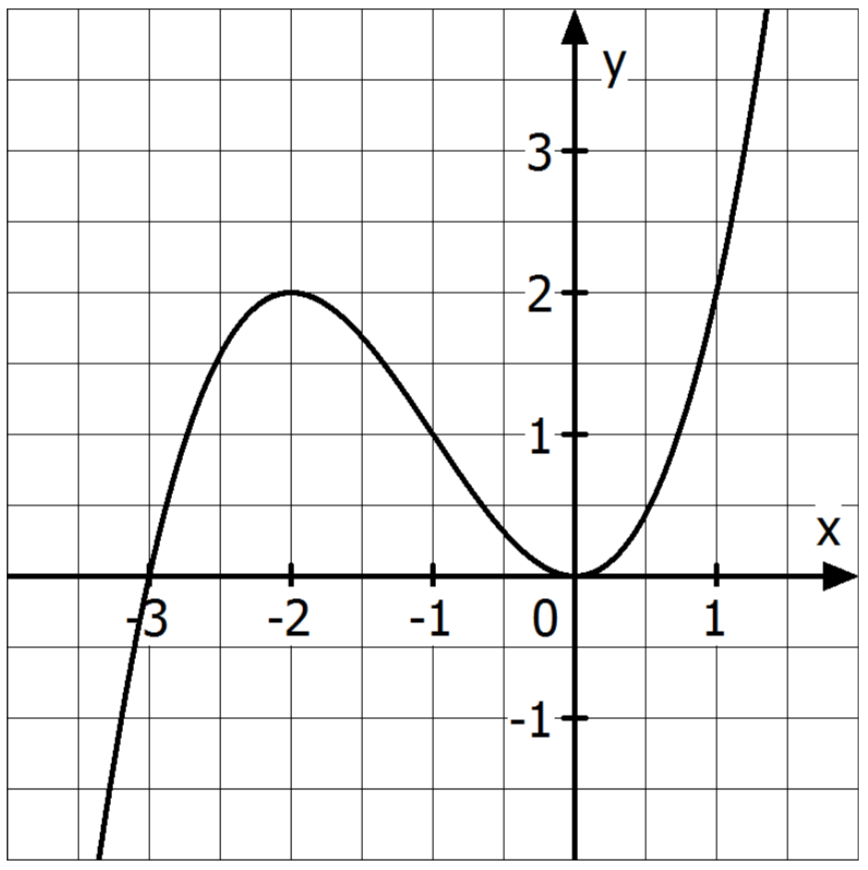
\includegraphics[width=0.7\linewidth]{Graphanalyse.png}
\end{multicols}

\begin{lsg}{}
	\begin{enumerate}
		\item Wahr, Vorzeichenwechsel bei $x=-3$
		\item Wahr, streng monoton steigend im Intervall $[-2;-1]$
		\item Falsch, $f''(-2)+f'(-2)=0+2>1$
		\item Wahr, $f'$ besitzt zwei Extrempunkte $\rightsquigarrow f''$ ist mindestens vom Grad 2. Der Graph der Abbildung könnte auch drei Nullstellen haben, $f'$ ist also mindestens vom Grad 3.
	\end{enumerate}
\end{lsg}





\aufgabe{Exponentialfunktion}
\begin{enumerate}
	\item Gib $f(x)=25^x$ als natürliche Exponentialfunktion an.
	\item	Wie unterscheidet sich der Graph von $-\e^{-x}$ von $\e^x$? Formuliere die Erklärung schrittweise.
\end{enumerate}
\begin{lsg}{}
	\begin{enumerate}
		\item $\e^{\ln(25)\cdot x}$
		\item 	\begin{itemize}
					\item $-\e^x$ ist zu $ \e^x$ an der x-Achse gespiegelt
					\item $\e^{-x}$ ist zu $\e^x$ an der y-Achse gespiegelt
				\end{itemize}
				$\Rightarrow -\e^{-x}$ ist zu $\e^x$ an der x- und der y-Achse gespiegelt
	\end{enumerate}
\end{lsg}


\aufgabe{Integral: }
Die Gerade $y=x$ und die $x$-Achse begrenzen zusammen mit den Geraden $x=2$ und $x=u$ mit $u>2$ eine Fläche. Bestimmen Sie einen Wert für $u$ so, dass $f(x)=x-\frac{8}{x^2}$ diese Fläche in zwei inhaltsgleiche Teile zerlegt. \cas
\begin{lsg}{}
  Bestimme die Flächeninhalte der Teilflächen:\begin{align*}
  A_1&=\int_2^u\left(x-\left(x-\frac{8}{x^2}\right)\right)\d x&&|\ \text{Fläche zwischen $y=x$ und $f(x)=x-\frac{8}{x^2}$}\\
  A_2&= \int_2^u\left(x-\frac{8}{x^2}\right)\d x&&|\ \text{Fläche zwischen $f(x)=x-\frac{8}{x^2}$ und $x$-Achse}
  \end{align*}
  Gleichsetzten und mittels CAS nach $u$ auflösen ergibt: $u\approx 3,12$
\end{lsg}



\aufgabe{Stammfunktion berechnen: } Berechne jeweils ein Stammfunktion zu den angegebenen Funktionen:
\begin{multicols}{3}
	\begin{enumerate}
		\item $f(x)=x^2+x-3$
		\item $f(x)=(2x-3)^8$
		\item $f(x)=-5\sin(3x+2)$
		\item $f(x)=\e^{3x+7}$
		\item $f(x)=\frac{1}{x*\ln x}$
		\item $f(x)=\e^{x-\e^x}$
	\end{enumerate}
\end{multicols}
\begin{lsg}{}
	\begin{multicols}{2}
		\begin{enumerate}
			\item $F(x)=\frac 1 3x^3+\frac 1 2 x^2-3x$
			\item $F(x)=\frac 1 9 (2x-3)*\frac 1 2=\frac{1}{18}(2x-3)$
			\item $F(x)=\frac 5 3 \cos(3x+2)$
			\item $F(x)=\frac 1 3 \e^{3x+7}$
			\item $f(x)=\frac 1 x*\frac{1}{\ln(x)}\rightsquigarrow F(x)=\ln(\ln x)$
			\item $f(x)=\e^x*\e^{-\e^x}\rightsquigarrow F(x)=-\e^{-\e^x}$
		\end{enumerate}
	\end{multicols}
\end{lsg}

\aufgabe{Rotationskörper: }
\begin{enumerate}
  \item Die Fläche, welche von der $x$-Achse und dem Graphen der Funktionen vollständig eingeschlossen wird, rotiert um die $x$-Achse.
  Berechne den Rauminhalt des entstandenen Körpers.
  \begin{itemize}
    \item $f(x)=x^2-2x$
    \item $g(x)=\sqrt{x}*(x-2)$
    \item $h(x)=\frac 1 3 x^2-x$
    \item $j(x)=x^2-5x+4$
  \end{itemize}
  \item Die Fläche, welche von den Graphen der Funktionen vollständig eingeschlossen wird, rotiert um die $x$-Achse.
  Berechne den Rauminhalt des entstandenen Körpers.
  \begin{itemize}
    \item $f(x)= -x^2+4, \quad g(x)= x+2$
    \item $h(x)= x^2-x+1, \quad j(x)= 4x-3$
  \end{itemize}
\end{enumerate}
\begin{lsg}{}
	\begin{enumerate}
		\item \begin{itemize}
			\item Nullstellen bei $x_0=0, x_1=2$
			\begin{equation*}
				V=\pi*\int\limits_0^2(x^2-2x)^2\d x =\frac {16\pi}{15}\approx 3,35
			\end{equation*}
			\item Nullstellen bei $x_0=0, x_1=2$
			\begin{equation*}
				V=\pi*\int\limits_0^2(\sqrt{x}*(x-2))^2\d x =\frac {4\pi}{3}\approx 4,18
			\end{equation*}
			\item Nullstellen bei $x_0=0, x_1=3$
			\begin{equation*}
				V=\pi*\int\limits_0^3(\frac 1 3 x^2-x)^2\d x =\frac {9\pi}{10}\approx 2,83
			\end{equation*}
			\item Nullstellen bei $x_0=1, x_1=4$
			\begin{equation*}
				V=\pi*\int\limits_1^4(x^2-5x+4)^2\d x =\frac {81\pi}{10}\approx 25,4
			\end{equation*}
		\end{itemize}
		\item \begin{itemize}
			\item Schnittpunkte bei $x_0=-2, x_1=1$
			\begin{equation*}
				V=\pi*\int\limits_-2^1\left((-x^2+4)-(x+2)\right)^2\d x =\frac {81\pi}{10}\approx 25,4
			\end{equation*}
			\item Schnittpunkte bei $x_0=1, x_1=4$
			\begin{equation*}
				V=\pi*\int\limits_1^4\left((4x-3)-(x^2-x+1)\right)^2\d x =\frac {81\pi}{10}\approx 25,4
			\end{equation*}
		\end{itemize}
	\end{enumerate}
\end{lsg}


\end{document}
